% fedOPD conference paper - draft generated 2026-07-30.
% Every result number in this document is transcribed from the stored result csvs in
% data/processed/ (via the tables regenerated from them on the draft date), never from memory;
% figures are the pngs generated by src/13_report_figures.ipynb from the same csvs.
\documentclass[conference]{IEEEtran}
\usepackage{graphicx}
\usepackage{booktabs}
\usepackage{amsmath}
\usepackage[hidelinks]{hyperref}
\graphicspath{{../../output/figures/}}

\title{fedOPD: Federated and Agentic Decision Support for NHS Waiting Lists ---\\
What Eight Years of Referral-to-Treatment Data Can and Cannot Predict}

\author{\IEEEauthorblockN{Nilesh Sarkar}
\IEEEauthorblockA{nileshsarkar.cs@gmail.com\\
Code, data pipeline and all stored outputs: \url{https://github.com/nileshsarkar-ai/fedOPD}}}

\begin{document}
\maketitle

\begin{abstract}
The English NHS elective waiting list grew from a monthly mean of 4.28 million pathways before
Covid-19 to 6.57 million after, while the share waiting over 52 weeks rose 81-fold (0.05\% to
4.11\%). Allocation decisions need forecasts at the provider--specialty level, but patient-level
data cannot be centralised freely. We build fedOPD, a fully audited pipeline over 96 months of
public Referral-to-Treatment (RTT) and KH03 bed data (343{,}441 provider--specialty--month rows,
651 providers), and evaluate demand forecasting, federated learning (FL) and rule-based allocation
agents under a pre-registered protocol: a sealed final year (FY~2025--26) declared before any model
was fit and read exactly once. On validation, naive persistence (MAE 153.5 on 1{,}407 rows at the
largest specialty) is unbeaten by nine model families at every spatial grain and horizon.
Level-space FedAvg fails on non-IID clients (MAE 186.5), but reformulating clients in
\emph{delta space} repairs federation completely: federated MAE 154.0 versus 153.8 for centralised
pooling, with a median gap of $-0.08$ MAE across 23 specialties --- collaboration without raw data
sharing at zero accuracy cost. A federated GRU gave the only sub-persistence validation scores
(150.6/152.4 vs.\ 154.1), confirmed across three declared seeds, yet on the sealed year persistence
retook the lead by 0.1 MAE while models won at 14--15 of 23 specialties; year-over-year drift in
persistence error (median $+4.6\%$) exceeds every model margin. We conclude that the deployable
product is calibrated uncertainty (conformal bands, 87.6--89.6\% empirical coverage) plus frozen
decision rules, with federation as a free privacy layer --- not a better point forecast.
\end{abstract}

\begin{IEEEkeywords}
federated learning; NHS waiting lists; demand forecasting; conformal prediction; agentic decision
support; healthcare resource allocation
\end{IEEEkeywords}

\section{Introduction}
Elective care in England is managed through Referral-to-Treatment (RTT) pathways, reported monthly
per provider and treatment function (specialty)~\cite{nhsrtt}. The post-pandemic backlog turned
these statistics into a planning instrument: integrated care boards (ICBs) must decide where to
expand capacity, when to redistribute demand, and when to buy independent-sector activity. Such
decisions implicitly assume the near future of each waiting list is predictable, and that the data
needed to predict it can be pooled. Both assumptions deserve measurement rather than faith.

Two obstacles stand out. First, hospital-level operational data is exactly the setting where
federated learning~\cite{mcmahan2017} is attractive --- organisations that cannot freely centralise
records could still train a shared model --- but hospitals are strongly non-IID clients: a teaching
trust and a specialist centre have waiting lists that differ by orders of magnitude, the regime in
which naive federated averaging is known to degrade~\cite{zhao2018,li2020}. Second, forecasting
literature repeatedly finds that simple benchmarks are hard to beat on noisy operational
series~\cite{makridakis2020,hyndman2021}; a federated model that loses to ``next month equals this
month'' is an expensive way to be wrong.

This paper reports fedOPD, an end-to-end study on eight years of public NHS data with the
discipline of a prospective trial. Our contributions are:
(i)~a fully audited 96-month panel joining RTT waiting lists to KH03 bed capacity, with every
documented number reproduced by asserts inside the notebooks that compute it;
(ii)~a baseline closure result: persistence is unbeaten on MAE by nine model families at every
grain (provider, ICB, national) and horizon (1--12 months) on a held-out validation year;
(iii)~a federation result: level-space FedAvg fails on non-IID hospitals, but delta-space
reformulation makes federated linear and near-federated neural clients match centralised pooling;
(iv)~frozen, ratified allocation rules whose simulated decisions separate real populations, together
with a structural finding that in-ICB-only redistribution is geographically starved; and
(v)~a one-shot sealed-year evaluation, pre-registered before execution, that adjudicates all of the
above prospectively.

\section{Related Work}
Federated averaging was introduced by McMahan et~al.~\cite{mcmahan2017}; its degradation under
non-IID client distributions is documented by Zhao et~al.~\cite{zhao2018}, with algorithmic
remedies such as FedProx~\cite{li2020} and a broad survey in Kairouz et~al.~\cite{kairouz2021}.
Healthcare is a canonical FL motivation: Rieke et~al.~\cite{rieke2020} argue for federation in
digital health, and Sheller et~al.~\cite{sheller2020} demonstrate multi-institutional model
training without data sharing. Most health-FL studies, however, evaluate against other learned
models rather than against operational naive baselines.

In forecasting, the M4 competition~\cite{makridakis2020} and standard texts~\cite{hyndman2021}
establish that naive and seasonal-naive benchmarks are frequently competitive on aggregate
operational series; queueing-based views of hospital waiting lists date back to
Worthington~\cite{worthington1987}, and policy analyses of waiting-time initiatives caution that
system dynamics dominate marginal predictive gains~\cite{kreindler2010}. For uncertainty, conformal
prediction provides distribution-free coverage guarantees~\cite{vovk2005,angelopoulos2023},
including regression variants~\cite{romano2019}. Our neural clients use standard components: gated
recurrent units~\cite{cho2014} trained with Adam~\cite{kingma2015}.

\section{Research Gap}
Three gaps motivate the study. (1)~Federated learning for health operations is rarely benchmarked
against the naive forecasts that practitioners already use, on public data anyone can audit.
(2)~Reported gains are seldom tested \emph{prospectively}; a sealed, pre-registered final year ---
standard in clinical research --- is almost absent from FL forecasting papers. (3)~Allocation
(``agentic'') rules are usually decoupled from the measured uncertainty of the forecasts that
trigger them. fedOPD addresses all three on one pipeline.

\section{Proposed Methodology}

\subsection{Data and panel construction}
We ingest all 96 monthly RTT ``full extract'' CSVs from April 2018 to March 2026~\cite{nhsrtt}
(schema break in April 2021 handled by name-derived band mapping), quarterly KH03 bed availability
and occupancy~\cite{nhskh03}, and the ODS trust reference. The canonical panel has 343{,}441
provider$\times$specialty$\times$month rows and 24 columns: waiting-list size, $>$18- and
$>$52-week counts and shares, trust metadata, ICB code, and general-and-acute occupancy. The
NHS-supplied aggregate row (\texttt{C\_999}) is excluded everywhere (its inclusion silently doubles
national totals); 651 providers appear, of which 193 public trusts hold 94.5\% of the list.
Fig.~\ref{fig:trend} shows the national series with the two declared epochs.

\begin{figure}[t]
\centering
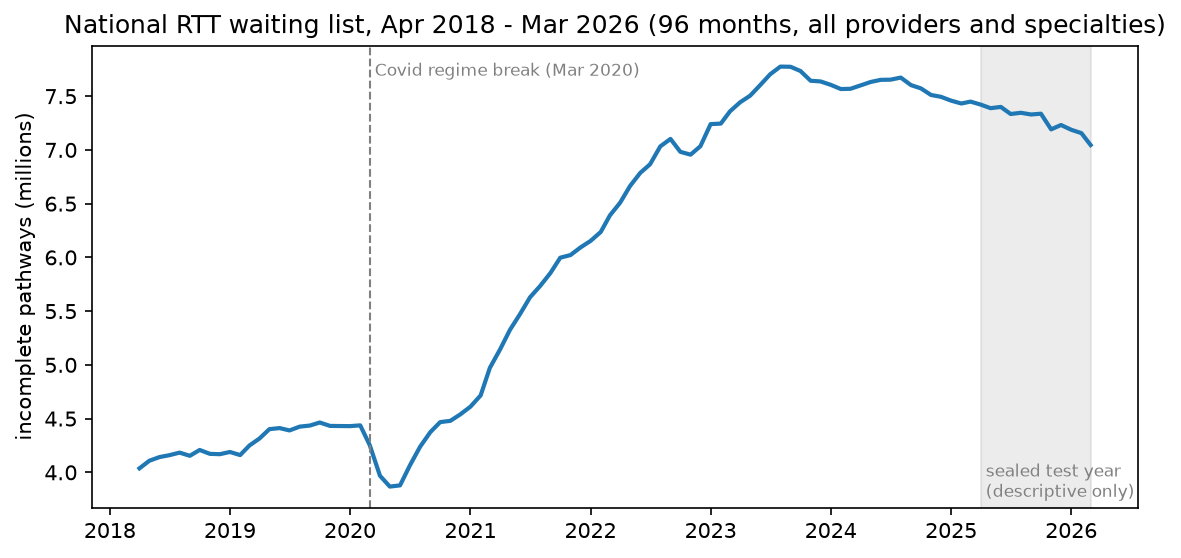
\includegraphics[width=\columnwidth]{fig_national_trend.png}
\caption{National RTT waiting list, Apr 2018--Mar 2026 (96 months, all providers and specialties).
The Covid regime break (Mar 2020) is the only regime boundary used anywhere; the shaded final year
is the sealed test set.}
\label{fig:trend}
\end{figure}

\textbf{Evaluation protocol, declared once.} The final fiscal year FY~2025--26 was sealed before
any model was fit: the development cut \texttt{month} $<$ 2025-04-01 is applied before target
construction, so sealed targets are unreachable by construction, and every modelling notebook
carries a sentinel assert on origin months. FY~2024--25 is the validation year. One seed (42) is
declared; the Covid break (March 2020) defines a ``post-only'' training regime evaluated alongside
full history. Nothing --- thresholds, splits, horizons --- was ever adjusted after seeing a metric.

\subsection{Forecasting layer and uncertainty}
The baseline is persistence, $\hat{y}_{t+h}=y_t$. Challengers on identical validation rows include
drift, seasonal-naive, gradient-boosted trees over lag/occupancy features, and referral-flow
(Part~3) covariates. Uncertainty is a split-conformal band~\cite{vovk2005}: with calibration
residuals $R=\{|y_{t+h}-y_t|\}$ from FY~2023--24, the band is $\hat{y}\pm q_{0.9}(R)$, giving
empirical validation coverage of 87.6--89.6\% (targets 90\%), from $\pm 298$ patients at $h{=}1$ to
$\pm 1{,}714$ at $h{=}12$.

\subsection{Federated clients}
Clients are providers within one specialty; the pool is the 149 public providers flagged
\texttt{fl\_client} ($\geq$48 months of history and reporting in the final month). We compare four
information regimes: local-only, centralised pooling, and federated averaging in two model spaces.
The level-space client is
\begin{equation}
\hat{y}_{t+1} = \beta_0 + \beta_1 y_t + \beta_2 (y_t - y_{t-1}),
\end{equation}
and the delta-space client is
\begin{equation}
\widehat{\Delta y}_{t+1} = a + b\,(y_t - y_{t-1}), \qquad \hat{y}_{t+1} = y_t + \widehat{\Delta y}_{t+1}.
\end{equation}
Both are exact least squares per client; federation is one sample-weighted coefficient average
\begin{equation}
\beta_{\mathrm{fed}} = \frac{\sum_k n_k\,\beta_k}{\sum_k n_k},
\label{eq:fedavg}
\end{equation}
so only two or three coefficients and a count ever leave a client.

The neural client is a single-layer GRU~\cite{cho2014} (input 4, hidden 32) with a linear head,
reading six-month windows of $(\log(1{+}y_t),\ \Delta y_t/100,\ s^{18}_t,\ s^{52}_t)$ ---
statistics-free transforms, so no scaler is fitted anywhere --- and predicting
$\Delta y_{t+1}/100$. Federation is classic FedAvg~\cite{mcmahan2017}: $R{=}10$ rounds of
broadcast, $E{=}5$ local full-batch Adam~\cite{kingma2015} steps (lr $10^{-3}$), then the
weighted average of Eq.~\eqref{eq:fedavg} applied to every weight tensor. The pooled reference
receives the identical total step budget ($R\times E = 50$ epochs). All hyperparameters were
declared a priori; there are no sweeps and no early stopping. Every model --- persistence
included --- is rescored on the identical window-eligible rows (at the anchor specialty
\texttt{C\_110}, 1{,}401 of the standard 1{,}407 validation rows), so no comparison ever mixes
denominators.

\subsection{Agent rules}
A provider-month pressure score is a weighted within-month percentile rank,
\begin{equation}
p_{it} = 0.2\,r_t(s^{18}_{it}) + 0.6\,r_t(s^{52}_{it}) + 0.2\,r_t(o_{it}),
\end{equation}
where $r_t(\cdot)$ ranks providers within month $t$ and $o$ is G\&A occupancy; the $>$52-week share
carries the largest weight because it is the component that moved 81-fold post-Covid. Rule set v1
combines pressure thresholds (0.70/0.40) with the 6-month conformal band (growth-risk
$1.20\times$, stability $1.05\times$) and occupancy slack (0.80); rule set v2 classifies
within-ICB senders and receivers by ICB-internal ranks ($\geq 0.80$ sender, $\leq 0.30$ receiver).
The constants were ratified and frozen on 2026-07-30; the freeze notebook re-derives all 2{,}337
simulated decisions from stored components and asserts bit-for-bit equality. A minimum receiver
group emerges arithmetically: a rank $\leq 0.30$ requires an ICB of at least
$\lceil 1/0.30 \rceil = 4$ providers.

\subsection{Sealed-year one-shot}
The final notebook is pre-registered in its own header before execution: full-history regime;
linear clients in two cuts (\emph{val-frozen} --- the exact validated fits --- and \emph{final} ---
refit on targets through March 2025); neural clients final-cut only at seed 42; test rows are
windows whose origin lies in FY~2025--26 (targets May 2025--March 2026). It ran exactly once; the
train/test split is asserted on target months, and the boundary window (origin March 2025) belongs
to neither set.

\section{Results and Discussion}

\subsection{The random walk is the forecast to beat --- and it wins}
On validation, persistence achieves MAE 153.5 (RMSE 330.1) over 1{,}407 provider-rows at
\texttt{C\_110} (Trauma \& Orthopaedics), and no challenger beats it: drift 157.4, GBM with flow
covariates 156.3 at $h{=}1$, widening with horizon (persistence 317.1/500.9/741.5 at
$h{=}3/6/12$); the same holds at ICB (310.2 at $h{=}1$) and national grain (3{,}777 at $h{=}1$).
Monthly persistence MAE ranges 123.3--221.9 across the validation year --- the target itself is
volatile, foreshadowing the sealed-year result.

\subsection{Federation is free in delta space}
Table~\ref{tab:fl} and Fig.~\ref{fig:flmodels} give the federation story. Naive level-space FedAvg
degrades badly on non-IID hospitals (186.5 full-history, 228.8 post-only) --- averaging intercepts
across providers of wildly different scale is the textbook failure~\cite{zhao2018}. The delta
reformulation removes the scale: federated 154.0 versus pooled 153.8, and across all 23 scored
specialties (26{,}504 validation rows) the federated-minus-pooled MAE gap has median $-0.08$
(worst $+1.27$, best $-4.61$). A delta model also edges persistence at 12 of 24 specialties
(largest margin \texttt{C\_120}: 165.1 vs.\ 171.6), showing the baseline closure above is
anchor-specific, though margins never exceed 6.5 MAE.

\begin{table}[t]
\caption{Validation MAE/RMSE at \texttt{C\_110}, identical 1{,}407 rows (\texttt{fl\_summary\_c110.csv}).}
\label{tab:fl}
\centering
\begin{tabular}{lcc}
\toprule
model & full history & post-Covid \\
\midrule
naive persistence & \textbf{153.5} / 330.1 & --- \\
pooled (centralised) & 153.8 / 330.3 & 155.4 / 331.9 \\
FedAvg, delta space & 154.0 / 332.0 & 155.5 / 333.1 \\
FedAvg, delta + local intercept & 155.3 / 334.3 & 157.4 / 336.3 \\
local-only (level space) & 161.9 / 345.2 & 166.5 / 350.5 \\
FedAvg, level space & 186.5 / 363.5 & 228.8 / 401.4 \\
\bottomrule
\end{tabular}
\end{table}

\begin{figure}[t]
\centering
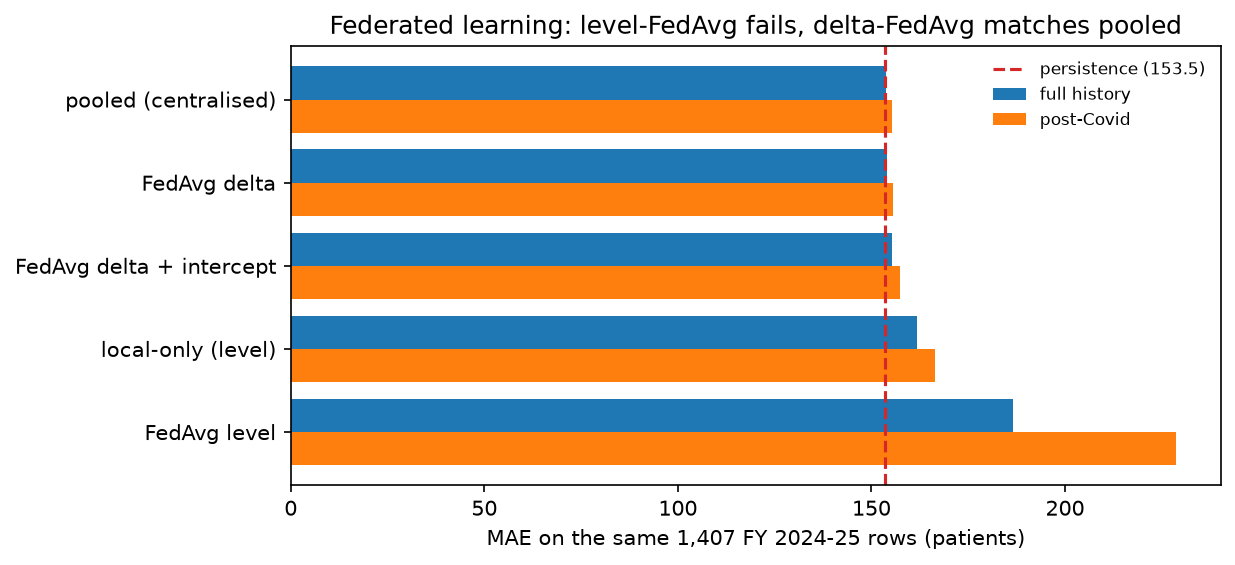
\includegraphics[width=\columnwidth]{fig_c110_fl_models_h1.png}
\caption{Level-space federation fails; delta-space federation matches centralised pooling
(validation, both regimes, same 1{,}407 rows).}
\label{fig:flmodels}
\end{figure}

\subsection{Neural clients: a coin flip, except at the anchor}
The federated GRU beats federated linear at 11 of 23 specialties (median gap $+0.15$ MAE) and at
55.2\% of 2{,}441 client--specialty pairs --- statistically a coin flip. Where signal exists,
federation costs neural models more than linear ones (\texttt{C\_120}: pooled 163.9 vs.\ FedAvg
168.6, linear FedAvg 165.5): averaging nonlinear weights loses more than averaging two
coefficients. The exception is the anchor (Fig.~\ref{fig:neural}): neural pooled 150.6 and neural
FedAvg 152.4 versus persistence 154.1 on 1{,}401 identical rows --- the only sub-persistence scores
in the project --- confirmed by a declared three-seed check (seeds 42/123/999: pooled
$151.5\pm0.9$, FedAvg $152.4\pm0.0$, all six full-regime scores below persistence). Dataset size
does not decide the winner: the correlation between specialty size and the relative neural--linear
gap is $r=0.128$ (Fig.~\ref{fig:size}), and the four largest relative neural wins are the
administrative X-codes --- exactly the specialties with no pre-Covid history. Even at its best the
delta signal is thin: the highest delta-space $R^2$ anywhere is $+0.075$.

\begin{figure}[t]
\centering
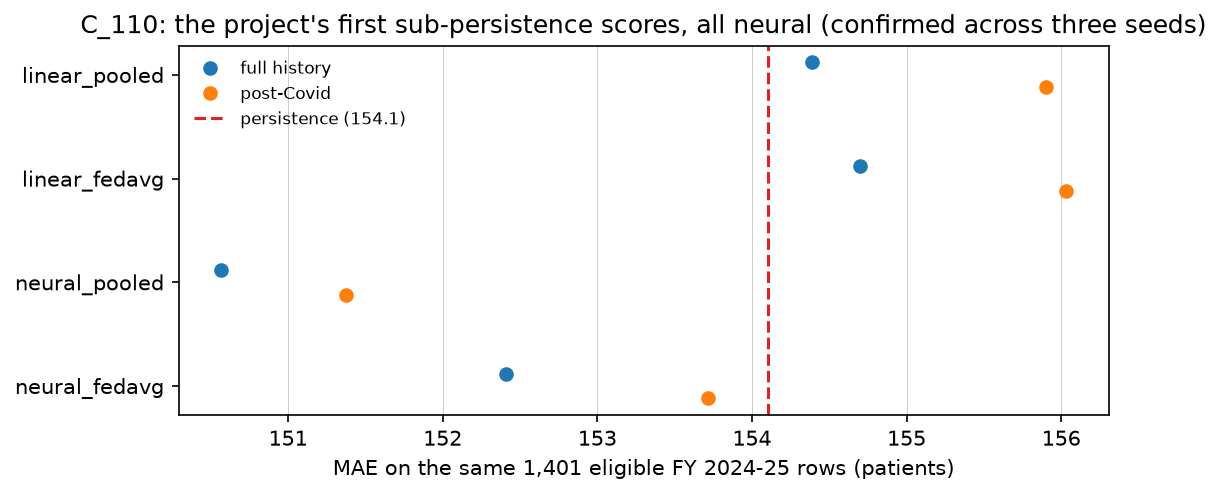
\includegraphics[width=\columnwidth]{fig_c110_fl_linear_vs_neural_h1.png}
\caption{Linear vs.\ neural families at \texttt{C\_110} on identical eligible rows (validation).}
\label{fig:neural}
\end{figure}

\begin{figure}[t]
\centering
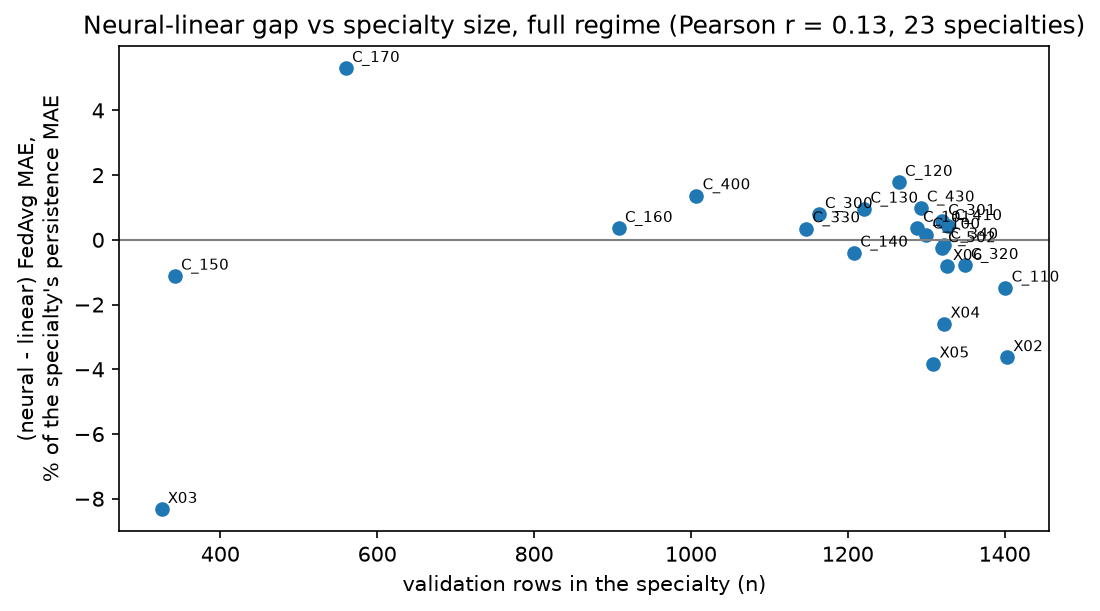
\includegraphics[width=\columnwidth]{fig_fl_neural_gap_vs_size_h1.png}
\caption{Relative neural--linear FedAvg gap vs.\ specialty size: $r=0.128$ --- size does not decide
the winner; the largest neural wins are the no-pre-Covid X-codes.}
\label{fig:size}
\end{figure}

\subsection{Covid regime: keep the history}
Once models are scale-free, discarding pre-Covid history hurts: full-history training beats
post-only at 17 of 18 clinical specialties for linear FedAvg and 15 of 18 for neural FedAvg
(Fig.~\ref{fig:covid}); the five X-codes sit exactly at zero (no pre-Covid rows to drop). The
largest penalty is \texttt{C\_502} ($+3.3$ MAE linear, $+2.4$ neural). The regime break that
dominates level models barely matters in delta space.

\begin{figure}[t]
\centering
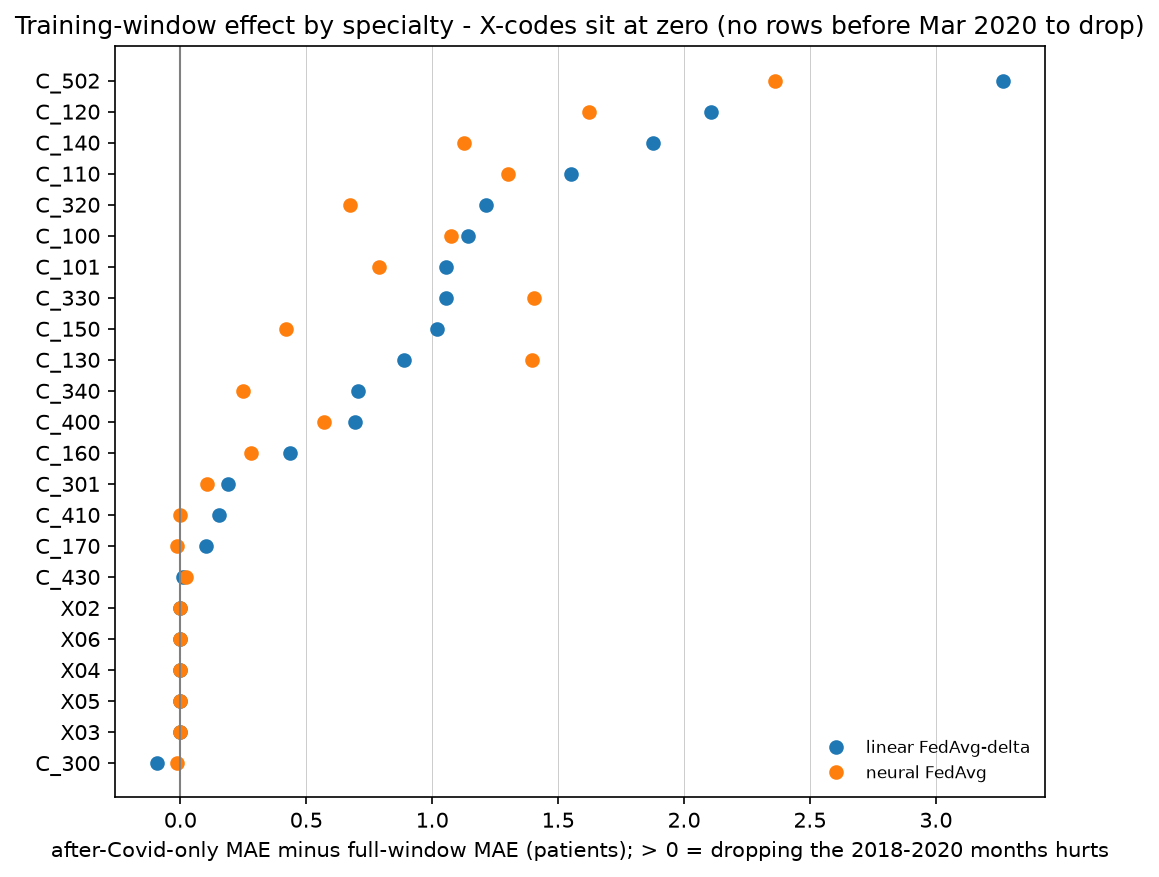
\includegraphics[width=\columnwidth]{fig_fl_covid_regime_effect_h1.png}
\caption{Cost of training on post-Covid data only (post minus full MAE), per specialty and family.}
\label{fig:covid}
\end{figure}

\subsection{Agent rules: clean signals, starved geography}
Over 2{,}337 provider-months (Apr 2023--Sep 2024, 132 providers), the frozen v2 rule flags 457
sender and 105 receiver months (median pressure 0.723 vs.\ 0.183; the separation is stable across
three disjoint 6-month stress windows: 0.764/0.717/0.673 vs.\ 0.179/0.181/0.198), and sender flags
precede the largest realised 6-month deteriorations (median $+81$ patients, $+181$ in the final
window). The structural finding is geographic: only 13.6\% of the 457 sender months have any
in-ICB receiver that month, and 246 of 457 (53.8\%) occur in ICBs with fewer than four cohort
providers, where a receiver is arithmetically impossible under the frozen threshold. In-ICB-only
redistribution is therefore starved by design; cross-ICB or independent-sector receiving is a
policy prerequisite, not a tuning choice. Rule set v1's receiver condition never fires (0 of
2{,}337) --- kept, documented, as evidence that band-conditioned receiving is too strict.

\subsection{The sealed year adjudicates}
Table~\ref{tab:sealed} and Fig.~\ref{fig:sealed} report the one-shot. At the anchor, persistence
retakes the lead: 151.5 versus neural pooled 151.6 ($n{=}1{,}407$) --- the three-seed-confirmed
validation edge did not replicate prospectively. Yet the broader pattern strengthened: neural
pooled beats persistence at 15 of 23 specialties, neural FedAvg and final-cut linear FedAvg at 14
(the exact validated linear fits at 10), with the largest win at \texttt{C\_330} (163.2 vs.\
171.5). The dominant effect is the year itself: per-specialty persistence MAE drifted by a median
$+4.6\%$ from validation to sealed year (range $-51.1\%$ to $+38.2\%$, Fig.~\ref{fig:drift}) ---
larger than any model-over-baseline margin measured anywhere in the project.

\begin{table}[t]
\caption{Sealed-year FY 2025--26 MAE at \texttt{C\_110} ($n{=}1{,}407$), with each model's
validation-year MAE beside it (\texttt{sealed\_year\_eval.csv}).}
\label{tab:sealed}
\centering
\begin{tabular}{lcc}
\toprule
model & sealed & validation \\
\midrule
persistence & \textbf{151.5} & 154.1 \\
neural pooled (final, seed 42) & 151.6 & 150.6 \\
neural FedAvg (final, seed 42) & 152.1 & 152.4 \\
linear pooled / FedAvg (final) & 153.0 / 153.0 & 154.4 / 154.7 \\
linear pooled / FedAvg (val-frozen) & 153.3 / 153.3 & same fits \\
\bottomrule
\end{tabular}
\end{table}

\begin{figure}[t]
\centering
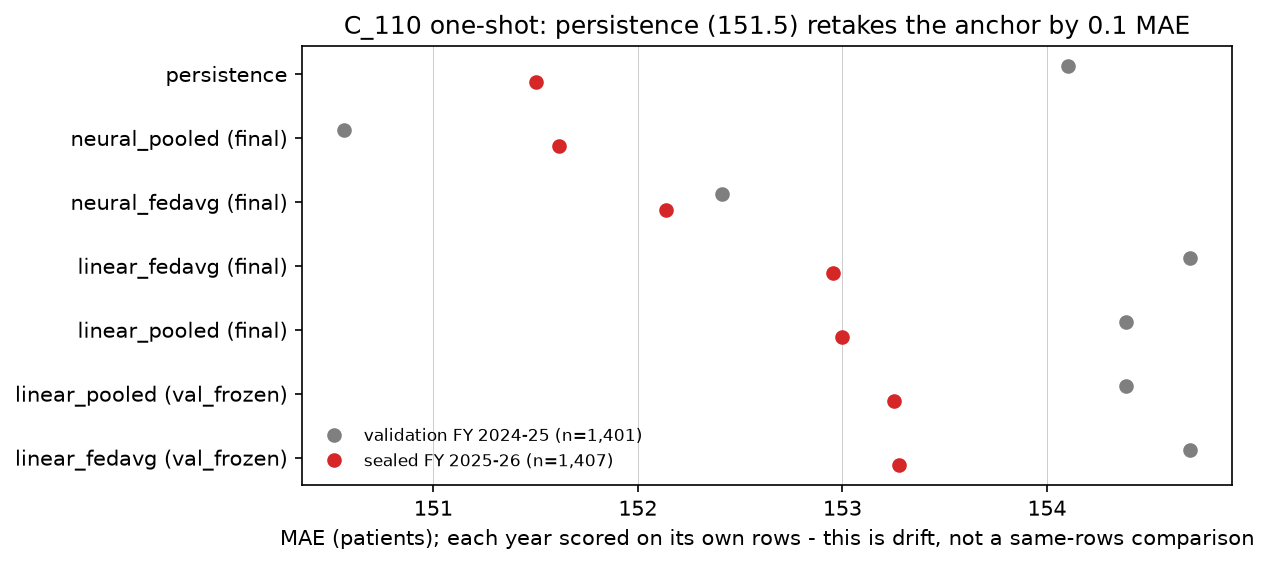
\includegraphics[width=\columnwidth]{fig_c110_sealed_one_shot_h1.png}
\caption{The one-shot verdict at the anchor: persistence retakes the lead by 0.1 MAE. Each year is
scored on its own rows (validation $n{=}1{,}401$, sealed $n{=}1{,}407$).}
\label{fig:sealed}
\end{figure}

\begin{figure}[t]
\centering
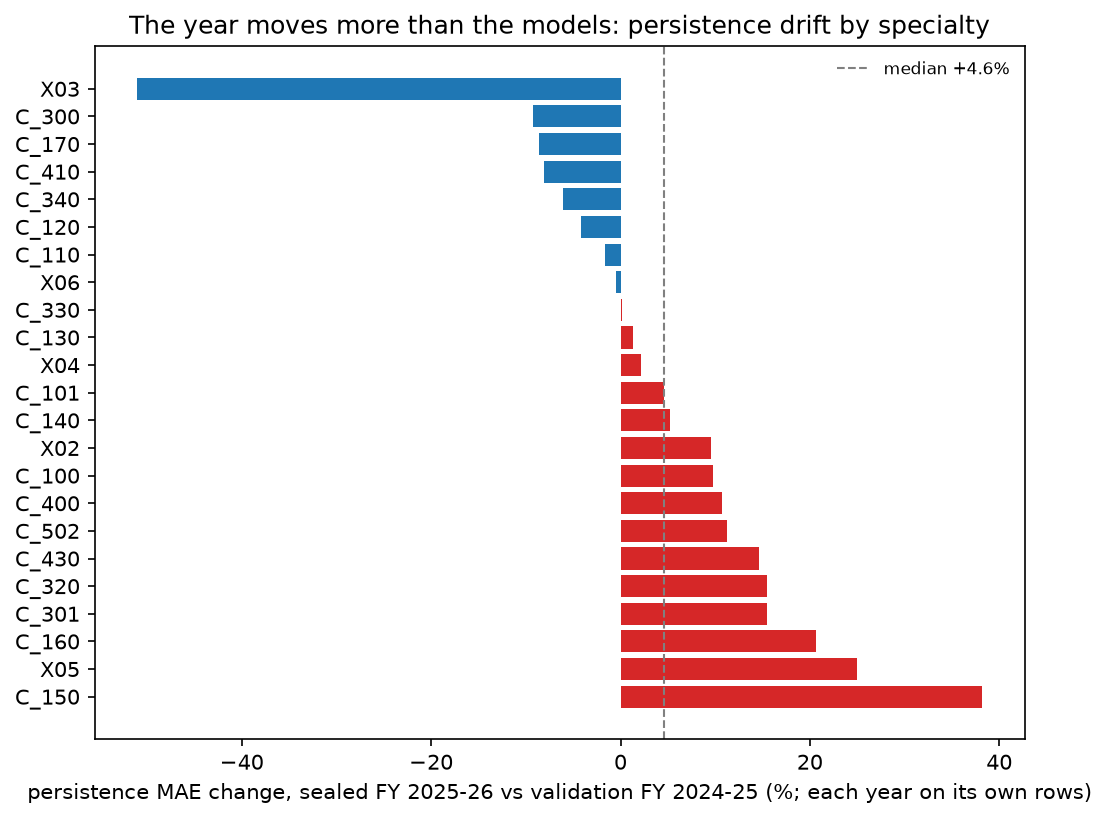
\includegraphics[width=\columnwidth]{fig_sealed_persistence_drift_h1.png}
\caption{Persistence MAE change from validation to sealed year, per specialty: the year moves more
than the models (median $+4.6\%$).}
\label{fig:drift}
\end{figure}

\subsection{Implications}
Three practical conclusions follow. First, \emph{federation is a free privacy layer}: in delta
space it costs essentially nothing relative to centralised pooling, so data-sharing agreements are
not a prerequisite for shared waiting-list models. Second, \emph{point-forecast improvements are
not where the value is}: sub-baseline margins of 1--3 MAE, even when seed-robust, did not survive a
prospective year whose own difficulty moved by $\pm$tens of percent; calibrated conformal bands
(87.6--89.6\% coverage) are the honest planning input. Third, \emph{allocation rules fail on
geography before they fail on statistics}: the frozen rules separate populations cleanly, but half
of all sender flags occur where no local receiver can exist --- widening the receiving pool matters
more than refining the score.

\section{Conclusion and Future Scope}
fedOPD demonstrates, on fully public data with a pre-registered sealed-year protocol, that
federated linear and neural clients can match centralised training at zero accuracy cost once
models predict changes rather than levels --- and that none of them reliably beats naive
persistence by more than a rounding error at any grain or horizon. The deployable system is
therefore persistence plus conformal uncertainty, frozen transparent allocation rules, and
federation as the privacy mechanism. Future work: widening the client pool to the 243
independent-sector \texttt{fl\_client} providers (RTT series without KH03 capacity); cross-ICB and
independent-sector receiving rules for the agent layer; richer exogenous signals (referral
pipelines, workforce); and FL algorithms beyond one-shot and FedAvg averaging (e.g.\
FedProx~\cite{li2020}) --- though the delta-space result suggests the binding constraint is signal,
not algorithm.

\begin{thebibliography}{17}
\bibitem{mcmahan2017} B.~McMahan, E.~Moore, D.~Ramage, S.~Hampson, and B.~A.~y~Arcas,
``Communication-efficient learning of deep networks from decentralized data,'' in \emph{Proc.
AISTATS}, 2017, pp. 1273--1282.
\bibitem{zhao2018} Y.~Zhao, M.~Li, L.~Lai, N.~Suda, D.~Civin, and V.~Chandra, ``Federated learning
with non-IID data,'' arXiv:1806.00582, 2018.
\bibitem{li2020} T.~Li, A.~K.~Sahu, M.~Zaheer, M.~Sanjabi, A.~Talwalkar, and V.~Smith, ``Federated
optimization in heterogeneous networks,'' in \emph{Proc. MLSys}, 2020.
\bibitem{kairouz2021} P.~Kairouz \emph{et al.}, ``Advances and open problems in federated
learning,'' \emph{Foundations and Trends in Machine Learning}, vol.~14, no.~1--2, 2021.
\bibitem{rieke2020} N.~Rieke \emph{et al.}, ``The future of digital health with federated
learning,'' \emph{npj Digital Medicine}, vol.~3, no.~119, 2020.
\bibitem{sheller2020} M.~J.~Sheller \emph{et al.}, ``Federated learning in medicine: facilitating
multi-institutional collaborations without sharing patient data,'' \emph{Scientific Reports},
vol.~10, no.~12598, 2020.
\bibitem{makridakis2020} S.~Makridakis, E.~Spiliotis, and V.~Assimakopoulos, ``The M4 competition:
100,000 time series and 61 forecasting methods,'' \emph{International Journal of Forecasting},
vol.~36, no.~1, pp. 54--74, 2020.
\bibitem{hyndman2021} R.~J.~Hyndman and G.~Athanasopoulos, \emph{Forecasting: Principles and
Practice}, 3rd~ed. Melbourne: OTexts, 2021.
\bibitem{worthington1987} D.~J.~Worthington, ``Queueing models for hospital waiting lists,''
\emph{Journal of the Operational Research Society}, vol.~38, no.~5, pp. 413--422, 1987.
\bibitem{kreindler2010} S.~A.~Kreindler, ``Policy strategies to reduce waits for elective care: a
synthesis of international evidence,'' \emph{British Medical Bulletin}, vol.~95, no.~1, pp. 7--32,
2010.
\bibitem{vovk2005} V.~Vovk, A.~Gammerman, and G.~Shafer, \emph{Algorithmic Learning in a Random
World}. New York: Springer, 2005.
\bibitem{angelopoulos2023} A.~N.~Angelopoulos and S.~Bates, ``Conformal prediction: a gentle
introduction,'' \emph{Foundations and Trends in Machine Learning}, vol.~16, no.~4, pp. 494--591,
2023.
\bibitem{romano2019} Y.~Romano, E.~Patterson, and E.~Cand\`es, ``Conformalized quantile
regression,'' in \emph{Proc. NeurIPS}, 2019.
\bibitem{cho2014} K.~Cho \emph{et al.}, ``Learning phrase representations using RNN
encoder--decoder for statistical machine translation,'' in \emph{Proc. EMNLP}, 2014.
\bibitem{kingma2015} D.~P.~Kingma and J.~Ba, ``Adam: a method for stochastic optimization,'' in
\emph{Proc. ICLR}, 2015.
\bibitem{nhsrtt} NHS England, ``Consultant-led Referral to Treatment waiting times data,''
\url{https://www.england.nhs.uk/statistics/statistical-work-areas/rtt-waiting-times/}, accessed
2026.
\bibitem{nhskh03} NHS England, ``Bed availability and occupancy data --- overnight (KH03),''
\url{https://www.england.nhs.uk/statistics/statistical-work-areas/bed-availability-and-occupancy/},
accessed 2026.
\end{thebibliography}

\end{document}
